\chapter{Future Works}
This section describes future work that could be conducted within the problem area. Some suggestions are related to our implementation, some are related to the research conducted using the prototype.
\section{Prototype related future works}

\subsection*{Client position in Virtual Reality}
Knowing where the client is in the garden, while the architect is building it, is something most of the test participants commented on. In addition to this some kind of marker could be installed to track where the client was in the VR world and that would show op on the acrylic plate for the architect to know exactly where the client was at that moment. This could possibly be achieved using a projector that would show the position and rotation of the client, without affecting the camera's detection ability of the marker patterns on the plate.

\subsection*{Making the prototype lighter and easier to handle}
Another way to ease our prototype is to make it lighter. Basically this would be using another more transportable VR unit, that doesn't need as much setup time as it do right now. Furthermore a better webcam would be preferred.\\
Regarding the box, it needs to be the right size for the camera used so that we don't have any parts on the acrylic plate where the marker wont show up in the VR world. The box itself would be made lighter and in a way that makes it easier to transport.

\subsection*{Drawing sections}
One problem with the current implementation is that it is impossible to do things like a flowerbed. During the usability test, one participant also remarked that the ability to a create custom shaped pond would be nice. The idea is reasonably simple; one can draw enclosed shapes on the plate. Placing a marker inside this will cause the entire shape to be filled with the marker's object. Rotating the flower would control the density of the objects in the shape. This could also be used to add things like tiled paths, or walls to the garden, making it look way more like a real garden. How the implementation could work can be seen in Figure \ref{fig:ftemarkers}, and \ref{fig:ftrmarkerslegend}. The old markers on the top are just due to the reuse of the old model.
\begin{figure}[H]
	\centering
	\begin{minipage}[b]{0.49\textwidth}
		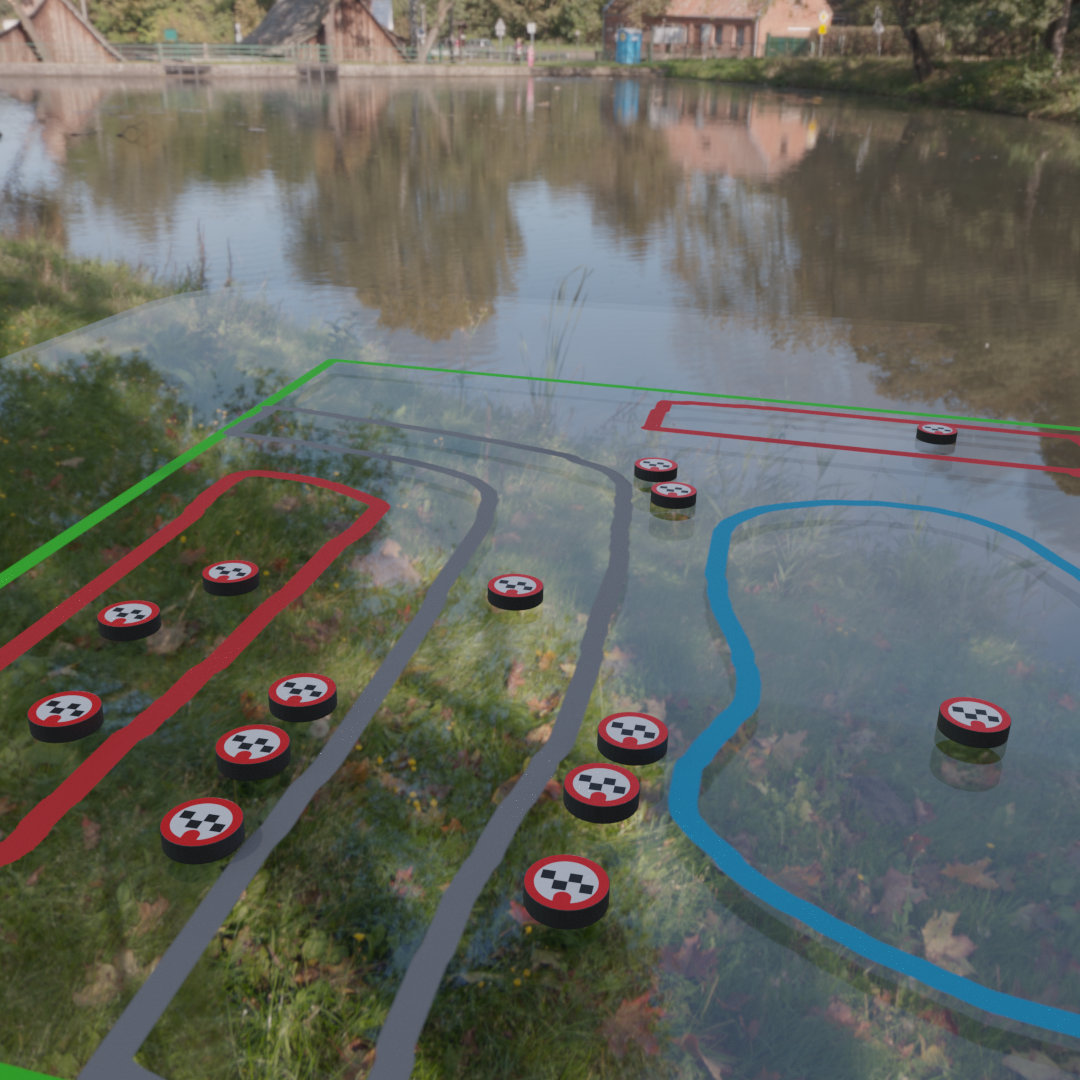
\includegraphics[width=1.0\linewidth]{figure/Evaluation/futuremarkers.png}
		\caption{Implementing this would allow architect to create flowerbeds, place multiple objects at a time, as well as change textures.}
		\label{fig:ftemarkers}
	\end{minipage}
	\hfill
	\begin{minipage}[b]{0.49\textwidth}
		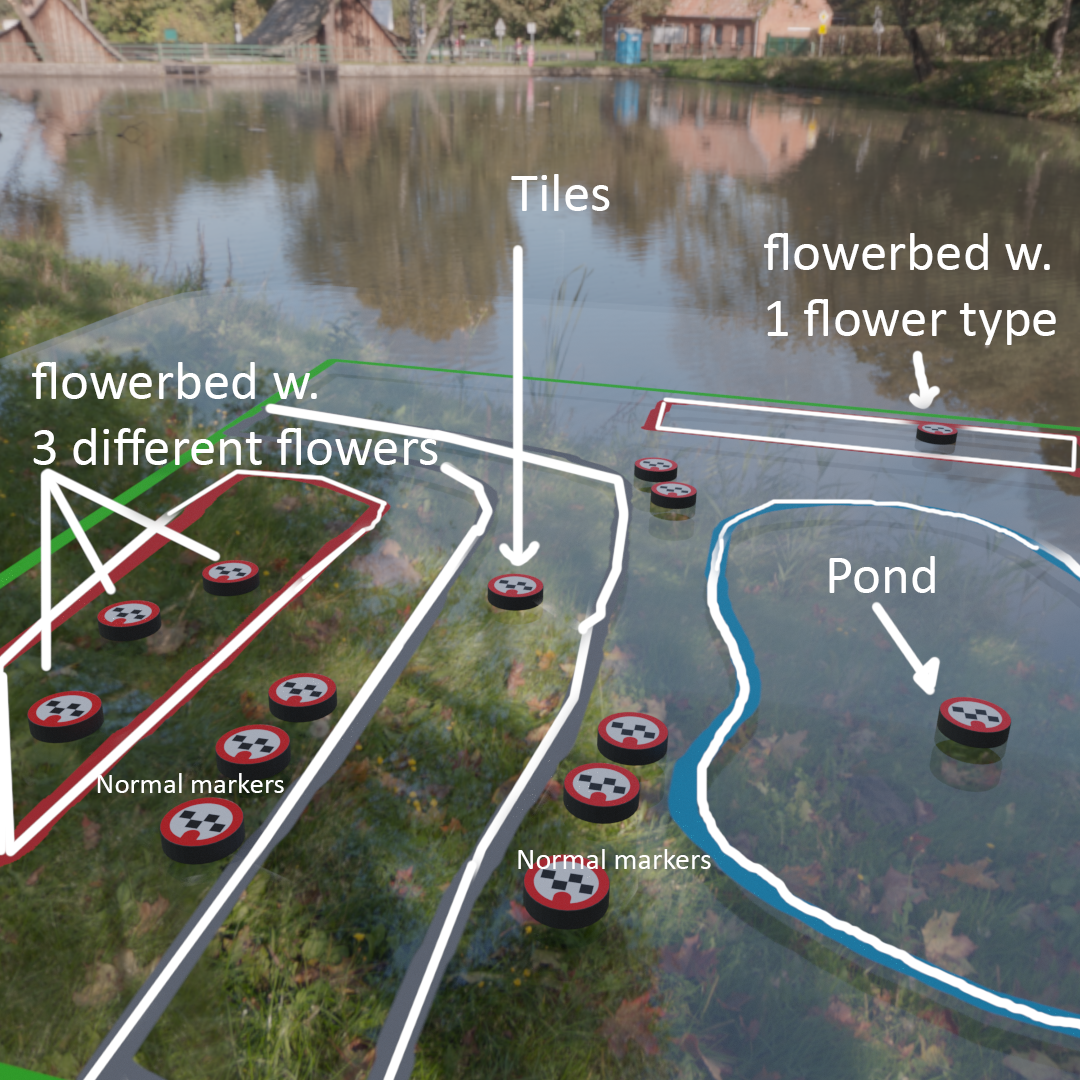
\includegraphics[width=1.0\linewidth]{figure/Evaluation/futuremarkerslegend.png}
		\caption{Explanation of what the Figure to the left would be interpreted as using this solution.}
		\label{fig:ftrmarkerslegend}
	\end{minipage}
\end{figure}

\subsection*{Adding the ability to export plant lists and measurements}
When the landscape architect and customer have agreed upon a final design there should to be an export functionality that gathers all the data from the tokens on the board and export plant lists and measurements etc. for the customer who can pass it on to a gardener and/or a paver as blueprints for their work.

\subsection*{Improving architect's ability to see orientation and relative size of objects}
The tests indicated that a garden architect working with our prototype would have a difficult time telling where objects were oriented, and how far apart to place tokens so that the virtual objects would not overlap. Small objects also could not be placed as close as was desirable due to the size of the physical tokens. The problem could be solved by using 3D printed tokens that match the look of the virtual objects, and ensuring that the rotation of the virtual object matches that of the token. The printed objects would then be scaled correctly relatively to each other, meaning that telling size would be intuitive. This would require smaller fiducial markers to accomodate the smallest 3D printed objects. As a consequence, storing the markers would take up significantly more space due to increased size and lack of stackability. 

\section{Evaluation related future work}

Better expert related research would be critical to establish the usefulness of the product inside the problem areas. Future researches should consider ways to get in contact with garden architects to ensure testers, as they proved an illusive target group.